\documentclass[border=10pt]{standalone} 
\usepackage[utf8]{inputenc}
\usepackage{nacal}
\usepackage{pgfplots}
\usepackage{tikz-3dplot}

\usepackage{tikz} 
\usetikzlibrary{matrix,decorations.pathreplacing}
% Añadida explícitamente arrows.meta para asegurar que Stealth funcione siempre
\usetikzlibrary{calc,angles,positioning,intersections,quotes,decorations.markings,arrows.meta}
\usepackage{tkz-euclide}

\pgfplotsset{width=10cm,height=6cm}

\begin{document}
  \def\Rojo{red!50!black}
  \def\RojoOscuro{red!20!black}
  \def\RojoClaro{red!90!black}
  \def\Verde{green!50!black}
  \def\VerdeOscuro{green!30!black}
  \def\VerdeClaro{green!50!gray}
  \def\Azul{blue!50!black}
  \def\AzulOscuro{blue!35!black}
  \def\AzulClaro{blue!60!gray}
  
  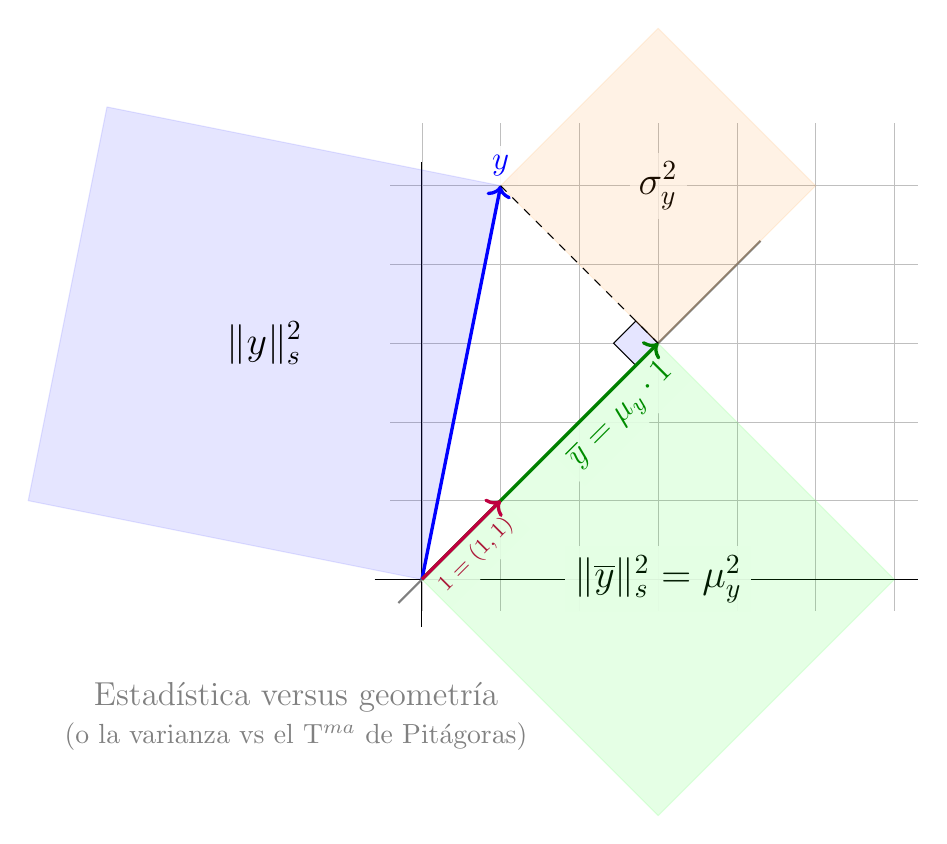
\begin{tikzpicture}
    
    % Definir los vectores
    \coordinate (O) at (0,0);            % Origen
    \coordinate (U) at (1,1);            % Vector Uno
    \coordinate (X) at (1,5);            % Vector de Datos
    % \coordinate (X) at (2,5);            % Vector de Datos
    
    % El código ($(O)!(X)!(U)$) significa: el punto de la recta que une (O) y (U) que está más cerca de (X)
    
    \coordinate (M) at ($(O)!(X)!(U)$);  % Vector mu * Uno.
    
    %%%%%%%%%%%%%%%%%%%%%%%%%%%%%%%%%%%%%%%%%%%%%%%%%%%% 
    %%%% Elementos por detrás de la figura principal %%%
    %%%%%%%%%%%%%%%%%%%%%%%%%%%%%%%%%%%%%%%%%%%%%%%%%%%% 
    
    % Dibujar cuadrícula 
    \draw[step=1cm,lightgray,very thin] (-.4,-.4) grid (6.3,5.8);
    % Dibujar ejes 
    \draw[-] (-.6,0) -- (6.3,0);   % eje x
    \draw[-] (0,-.6) -- (  0,5.3); % eje y
    
    % Etiquetas de los vectores x y mu*Uno
    \node[blue, right, fill=white,opacity=.9,text opacity=1] at (X) [above]{\large$\boldsymbol{y}$};
    \node[green!50!black,rotate=45,below left, fill=white,opacity=.9,text opacity=1] at (M) {\large$\boldsymbol{\mathop{\overline{y}}}=\mu_{\boldsymbol{y}}\cdot\boldsymbol{1}$};
    \node[purple,rotate=45,below,fill=white,opacity=.9,text opacity=1]  at ($(O)!0.5!(U)$) {\footnotesize$\boldsymbol{1}=(1,1)$};
    
    \node[gray]  at (-1.6,-1.5) {\large Estadística versus geometría};
    \node[gray]  at (-1.6,-2) {(o la varianza vs el T$^{ma}$ de Pitágoras)};
    
    
    % Dibujar la recta generada por el vector (1,1)
    \draw[-,thick,gray] (-.3,-.3) -- (4.3,4.3) node[right]{};
    
    % Marca de ángulo recto
    \tkzMarkRightAngle[fill=blue!10,size=.4](O,M,X)
    
    %%%%%%%%%%%%%%%%%%%%%%%%%%%%%%%%%%%%%%%%%%%%%%%%%%%% 
    %%%% Cuadrados de las longitudes %%%%%%%%%%%%%%%%%%%
    %%%%%%%%%%%%%%%%%%%%%%%%%%%%%%%%%%%%%%%%%%%%%%%%%%%% 
    
    % Varianza
    \tkzDefSquare(X,M); 
    \path (X) -- (tkzFirstPointResult) node[midway,fill=white,opacity=.7,text opacity=1] {\Large$\sigma_{\boldsymbol{y}}^2$};
    \tkzDrawPolygon[thin, orange, fill=orange,opacity=.1](X, M, tkzFirstPointResult, tkzSecondPointResult)
    % \path (tkzSecondPointResult) -- (tkzFirstPointResult) node[midway,sloped,purple,above] {\slshape $\boldsymbol{\lambda}$aura};
    
    % Cuadrado de la longitud de x
    \tkzDefSquare(O,X); \tkzDrawPolygon[thin, blue, fill=blue,opacity=.1](O, X, tkzFirstPointResult, tkzSecondPointResult)
    \path (O) -- (tkzFirstPointResult) node[midway,text opacity=1] {\Large$\|\boldsymbol{y}\|_s^2$};
    % \path (tkzSecondPointResult) -- (O)  node[midway,sloped,green!50!black,below] {\slshape $\boldsymbol{\beta}$ujos$\alpha$};
    
    % Cuadrado de la longitud de mu*Uno
    \tkzDefSquare(M,O);
    \path (M) -- (tkzFirstPointResult) node[midway,fill=white,opacity=.95,text opacity=1] {\Large$\|\boldsymbol{\mathop{\overline{y}}}\|_s^2=\mu_{\boldsymbol{y}}^2$};
    \tkzDrawPolygon[thin, green, fill=green,opacity=.1](M, O, tkzFirstPointResult, tkzSecondPointResult)
    % \path (tkzSecondPointResult) -- (tkzFirstPointResult) node[midway,sloped,blue,below] {\slshape $\delta$el Río};
    
    % DIBUJAR LOS VECTORES
    % Dibujar el vector X
    \draw[->,very thick, blue] (O) -- (X); % node[above,fill=white,opacity=.9,text opacity=1]{$\boldsymbol{y}$};
    
    % Dibujar el vector mu * Uno
    \draw[->,very thick,green!50!black] (O) -- (M); % node[right, fill=white,opacity=.9,text opacity=1]{$\mu\boldsymbol{1}$};
    
    % Dibujar la línea punteada entre X y mu*Uno
    \draw[dashed] (X) -- (M);
    
    % Dibujar el vector Uno
    \draw[->,very thick, purple] (O) -- (U); % node[sloped,midway,below,fill=white,opacity=.5,text opacity=1]{$\boldsymbol{1}=(1,1)$};
    
  \end{tikzpicture}
\end{document}
